\begin{frame}{\lexi{Avoir l'air} ou \lexi{rendre}?}
  Avec un.e partenaire, écrivez des phrases à partir des fragments donnés.
  Utilisez soit l'expression \lexi{avoir l'air} soit l'expression \lexi{rendre}.
  \begin{columns}
    \small
    \column{0.65\textwidth}
      \begin{enumerate}
        \item[] \textbf{Modèle:} \emph{Les avenues // encombré}
        \item[] \emph{Les avenues ont l'air encombrées.}
        \item \only<1>{Le bruit des villes // la vie // stressant}
              \only<2->{Le bruit des ville \alert{rend} la vie stressant\alert{e}.}
        \item \only<-2>{Les parcs // bien entretenu}
              \only<3->{Les parcs \alert{ont l'air} bien entretenu\alert{s}.}
        \item \only<-3>{Une famille bruyante peut // la vie en appartement // impossible}
              \only<4->{Une famille bruyante peut \alert{rendre} la vie en appartement impossible.}
        \item \only<-4>{La vie culturelle à Lyon // plus passionnant // qu'en province}
              \only<5->{La vie culturelle à Lyon \alert{a l'air} plus passionnant\alert{e} qu'en province.}
        \item \only<-5>{Les distractions // les grandes villes // stimulant}
              \only<6->{Les distractions \alert{rendent} les grandes villes stimulant\alert{es}.}
        \item \only<-6>{Les boulevards // animé // le soir}
              \only<7->{Les boulevards \alert{ont l'air} animé\alert{s} le soir.}
      \end{enumerate}
    \column{0.35\textwidth}
      \begin{minipage}[c][0.6\textheight]{\linewidth}
        \scriptsize
        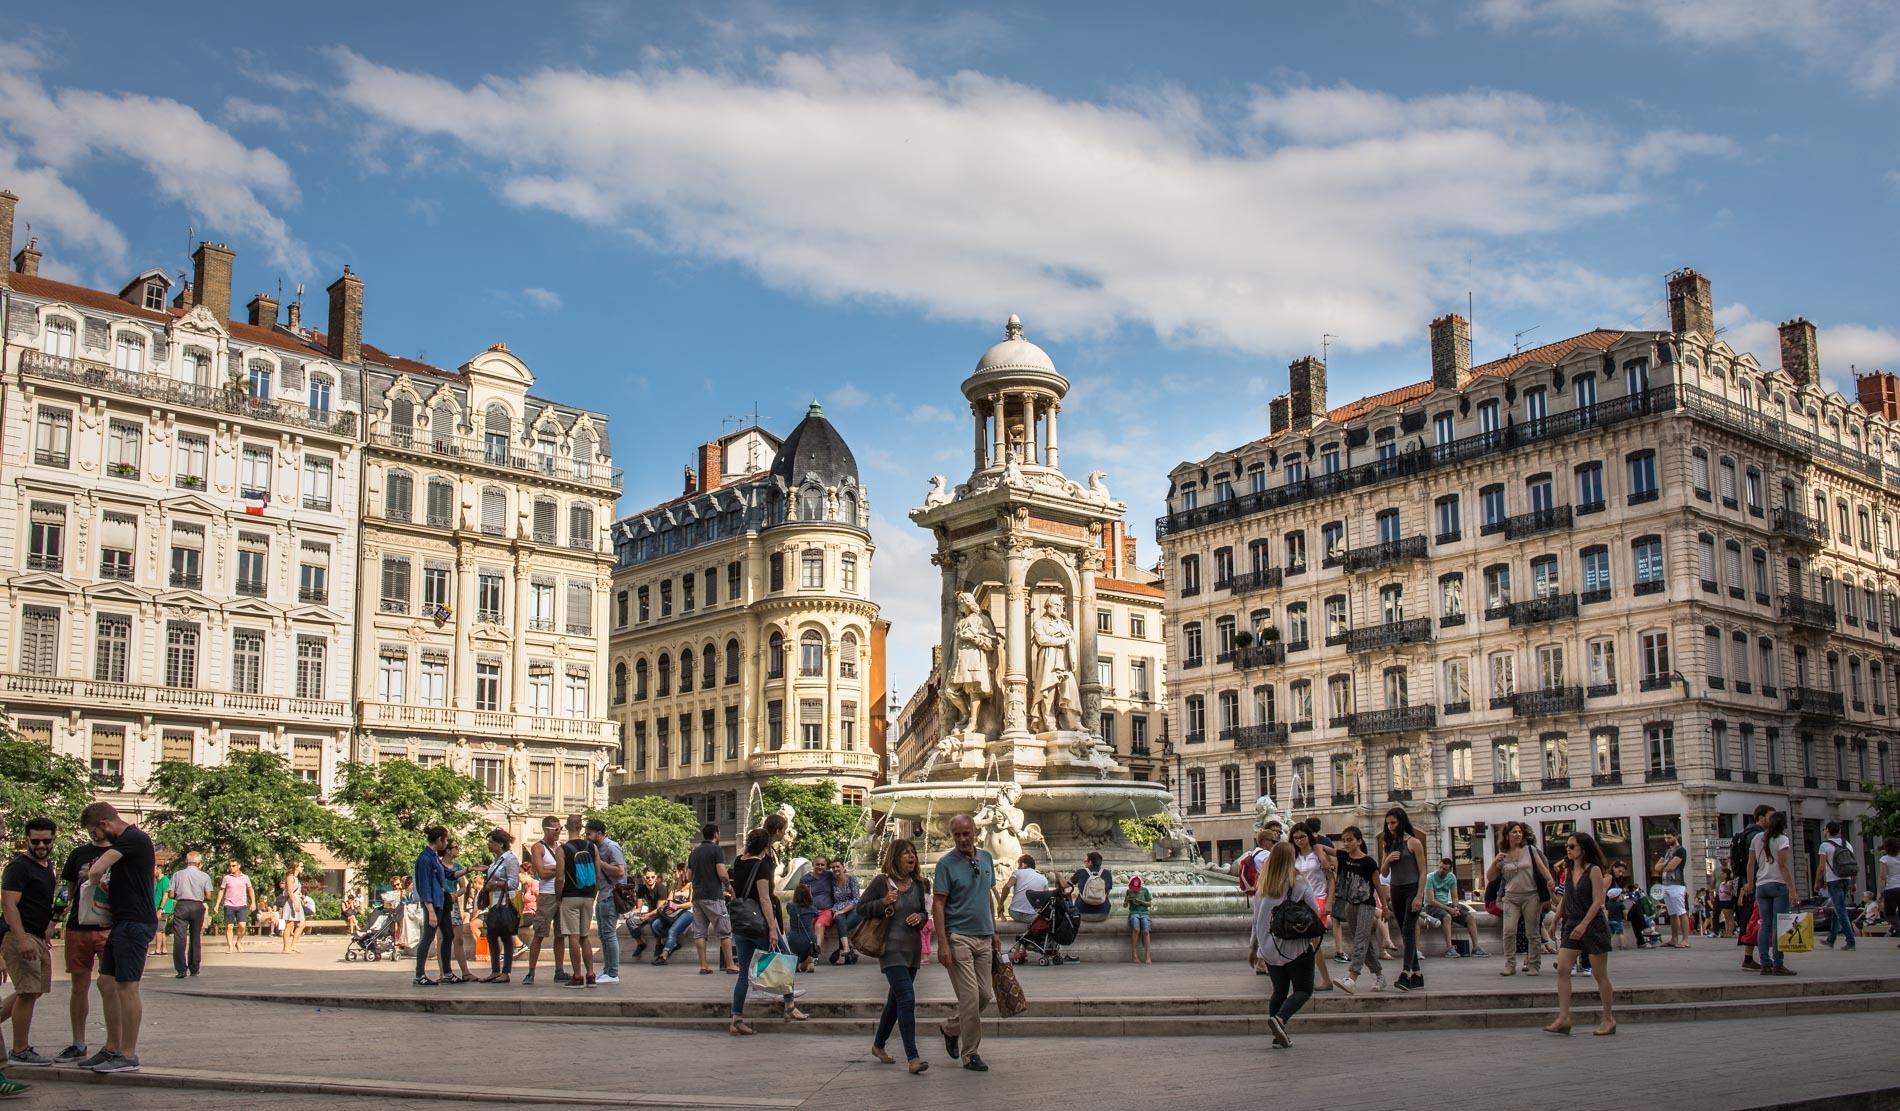
\includegraphics[scale=0.09]{lyon_centre_ville.jpg} \\
        Le centre-ville de Lyon
      \end{minipage}
  \end{columns}
\end{frame}